\documentclass[11pt]{exam}
\usepackage{graphicx} % Required for inserting images
\usepackage{amssymb}
\usepackage{amsmath}
\usepackage{optidef}
\usepackage{listings}
\usepackage{xcolor} % for custom colors
\usepackage{minted} % for code
\usepackage[T1]{fontenc}

% === Make things tighter ===
\usepackage[margin=0.75in]{geometry} % <- widen/narrow by changing 1.25in
\usepackage{setspace}
% \setstretch{0.95} % line spacing
\usepackage{enumitem}
% \setlist{nosep}  % removes vertical space around lists
% \setlist[itemize]{topsep=3pt, itemsep=3pt, parsep=1pt, partopsep=0pt}
% \setlist[enumerate]{topsep=3pt, itemsep=3pt, parsep=1pt, partopsep=0pt}
\usepackage{titlesec}
% \titlespacing*{\section}{0pt}{4.0ex plus 0.5ex minus 0.5ex}{0.8ex}
% \titlespacing*{\subsection}{0pt}{3.0ex plus 0.3ex minus 0.3ex}{0.6ex}
% \titlespacing*{\subsubsection}{0pt}{2.0ex plus 0.2ex minus 0.2ex}{0.4ex}
% \titlespacing*{\paragraph}{0pt}{1.5ex plus 0.2ex minus 0.2ex}{0.4ex}
\newcommand{\todo}[1]{\textit{\textcolor{orange}{ [#1]}}}


\lstset{
  language=Python,
  basicstyle=\ttfamily\scriptsize,
  keywordstyle=\color{blue},
  stringstyle=\color{red},
  commentstyle=\color{gray},
  showstringspaces=false,
  frame=single,
  breaklines=true
}
\title{6.S974 Games, Learning, and Security}
\author{Erich Trieschman}
\date{\today}
\begin{document}
\maketitle

\begin{questions}
    \question \textbf{Relief logistics.}
    \begin{parts}
        \part \textit{Min-cost flow problem.} Noticing that there's more available supply than demand, we introduce a "surplus" node $s$ that demands $100 = 1000 - 900$ to balance the problem.

        \textbf{Constants}
        \begin{align*}
            b &= [b_{c1}, b_{c2}, b_w, b_{d1}, b_{d2}, b_{s}]\\ 
              &= [-200, -700, 0, 400, 600, -100] \in \mathbb R^6\\
            c &= [c_{d1\to c1}, c_{d1\to c2}, c_{d1\to w},
                c_{d2\to c1}, c_{d2\to c2}, c_{d2\to w},
                c_{w\to c1}, c_{w\to c2}, c_{d1\to s}, c_{d2\to s}]\\
                &= [30,30,15,50,23,15,11,14, 0, 0] \in\mathbb R^{10}
        \end{align*}
        \textbf{Variable}
        \begin{align*}
            f &= [f_{d1\to c1}, f_{d1\to c2}, f_{d1\to w},
                f_{d2\to c1}, f_{d2\to c2}, f_{d2\to w},
                f_{w\to c1}, f_{w\to c2}, f_{d1\to s}, f_{d2\to s}] \in \mathbb R^{10}
        \end{align*}
        \textbf{Linear program}
        \begin{align*}
            \min_f\quad& 30f_{d1\to c1} + 30f_{d1\to c2} +15f_{d1\to w} +50f_{d2\to c1} +23f_{d2\to c2}\\[-0.5em]
            & +15f_{d2\to w}+ 11f_{w\to c1}+14f_{w\to c2} + 0f_{d1\to s} +0f_{d2\to s}\\[1em]
            \text{s.t.}\quad& 
            f_{d1\to c1} + f_{d2\to c1} + f_{w\to c1} = 200 \tag{Community 1}\\
            & f_{d1\to c2} + f_{d2\to c2} + f_{w\to c2} = 700 \tag{Community 2}\\
            &f_{d1\to w} + f_{d2\to w} = f_{w\to c1}+f_{w\to c2} \tag{Warehouse}\\
            &400 = f_{d1\to c1} + f_{d1\to c2} + f_{d1\to w} + f_{d1\to s} \tag{Depot 1}\\
            &600 = f_{d2\to c1} + f_{d2\to c2} + f_{d2\to w} + f_{d2\to s} \tag{Depot 2}\\
            &f_{d1\to s} + f_{d2\to s} = 100 \tag{Surplus}\\
            & f \succeq 0 \tag{Nonnegativity}
        \end{align*}
        \textbf{Directed network drawing.} See Figure~\ref{fig:1-a}
        \begin{figure}[htbp]
            \centering
            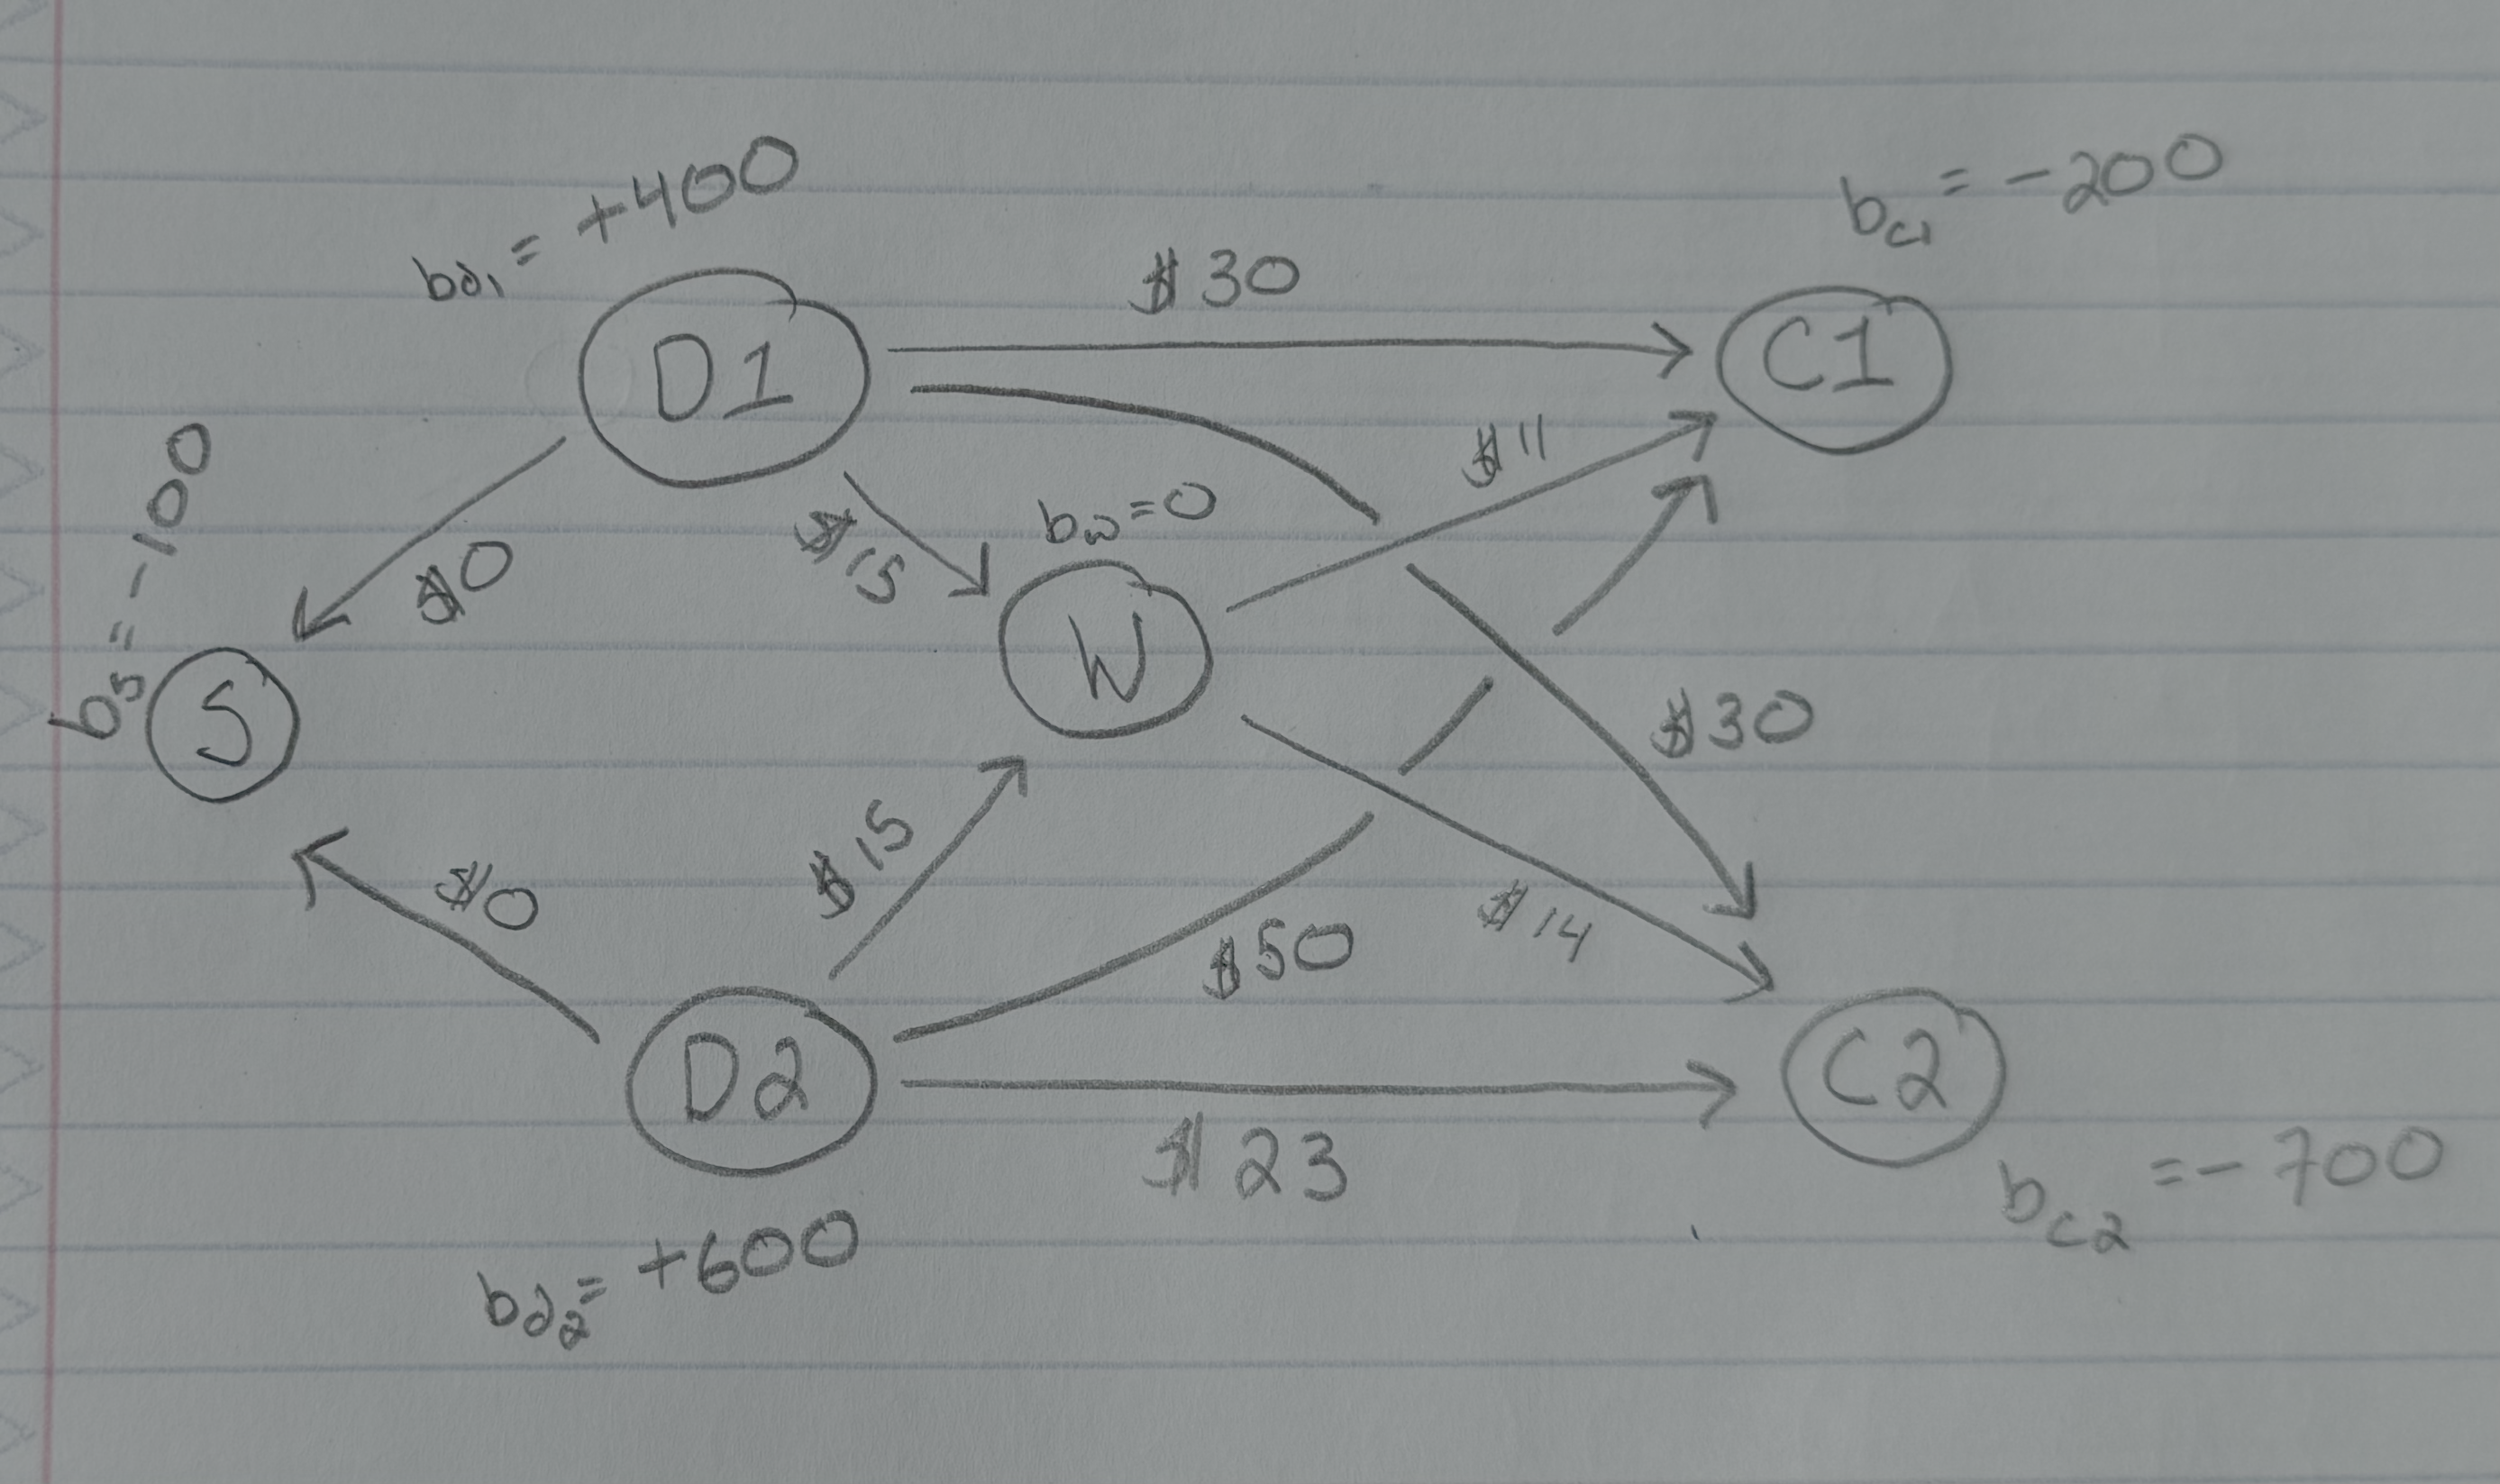
\includegraphics[width=0.6\textwidth]{hw1_problem1_parta.png}
            \caption{Problem 1 Part (a) directed network drawing}
            \label{fig:1-a}
        \end{figure}

        \part \textit{Fully loaded containers.} Yes the problem above admits a solution satisfying the constraint on fully loaded containers:
        \begin{enumerate}
            \item Scale the problem so supply, flows, demand, and costs are per 10 units:
            \begin{align*}
                b = [-20, -70, 0, 40, 60, -10],\quad
                c = [300,300,150,500,230,150,110,140, 0, 0]
            \end{align*}
            \item Integrality theorem says min-cost flow problem admits an integer optimal solution if i) the problem has an optimal and ii) $(b, u)\in \mathbb Z^{|n|}\times \mathbb Z^{|f|}$. Our problem satisfies i) as seen in part (d) and ii) since $b\in\mathbb Z^{|n|}$ is satisfied after problem scaling and since flows are only restricted to be nonnegative.
            \item An integer solution after scaling represents a solution in increments of 10, i.e., fully loaded containers.
        \end{enumerate}


        \part \textit{Extreme events.} First we introduce new variables $x_{c1}, x_{c2}$ to capture the amount of supply delivered to communities 1 and 2 respectively. We add corresponding constraints to limit delivered supply to be non-negative and to not exceed community demand. 
        We then formulate the objective of maximum unment demand, defined as
        \begin{align*}
            \max \Big\{1 - \tfrac{x_{c1}}{500}, 1 - \tfrac{x_{c2}}{700}\Big\}.
        \end{align*}
        Then we introduce epigraph variable $z$ to reformulate the maximum in the objective as epigraph constraints. We add additional constraints on the shipment budget and capacitated flows from the warehouse to community 1. We also drop the surplus node and corresponding constraints. The final linear program is
        \begin{align*}
            \min_{f,\mathcolor{red}{x, z}}\quad& \mathcolor{red}{z}\\
            \text{s.t.}\quad& 
            f_{d1\to c1} + f_{d2\to c1} + f_{w\to c1} \mathcolor{red}{=x_{c1}} \tag{Community 1}\\
            & f_{d1\to c2} + f_{d2\to c2} + f_{w\to c2} \mathcolor{red}{=x_{c2}} \tag{Community 2}\\
            &f_{d1\to w} + f_{d2\to w} = f_{w\to c1}+f_{w\to c2} \tag{Warehouse}\\
            &400 \mathcolor{red}{\geq} f_{d1\to c1} + f_{d1\to c2} + f_{d1\to w} \tag{Depot 1; unused supply allowed}\\
            &600 \mathcolor{red}{\geq} f_{d2\to c1} + f_{d2\to c2} + f_{d2\to w} \tag{Depot 2; unused supply allowed}\\
            & f \succeq 0 \tag{Nonnegativity}\\
            &\mathcolor{red}{f_{w\to c1}\leq 200} \tag{Capacitated flow}\\
            &\mathcolor{red}{0\leq x_{c1}\leq 500,\; 0\leq x_{c2}\leq 700} \tag{Deliveries can't exceed demand}\\
            &\mathcolor{red}{30f_{d1\to c1} + 30f_{d1\to c2} +15f_{d1\to w} +50f_{d2\to c1} +23f_{d2\to c2} +15f_{d2\to w}+ 11f_{w\to c1}+14f_{w\to c2} \leq 23000} \tag{Budget constraint}\\
            & \mathcolor{red}{1 - \tfrac{1}{500}x_{c1} \leq z,\; 1 - \tfrac{1}{700}x_{c2} \leq z} \tag{Reformulated max in objective}
        \end{align*}
        \part \textit{In code.} Supply can remain unused while demand is unmet because constraints on the total budget and on flows between the warehouse and community 1. 
        Specifically, restricting $w \to c1$ redirects flows to either $d1\to c1$ at an incremental cost of $+4 = 30 - (15 + 11)$ or $d2\to c1$ at an incremental cost of $+24 = 50 - (15 + 11)$. 
        Relaxing either the budget or the flow constraint would allow us to meet more unment demand with our unused supply. 
        \begin{lstlisting}[language=Python]
import numpy as np
import cvxpy as cp

# =======================
# Problem 1 Part (a)
# =======================
# constants
nodes = np.array(["C1", "C2", "W", "D1", "D2", "S"])
arcs = np.array(
    [
        "D1->C1",
        "D1->C2",
        "D1->W",
        "D2->C1",
        "D2->C2",
        "D2->W",
        "W->C1",
        "W->C2",
        "D1->S",
        "D2->S",
    ]
)
b = np.array([-200, -700, 0, 400, 600, -100])
c = np.array([30, 30, 15, 50, 23, 15, 11, 14, 0, 0])
A = np.array(
    [
        [-1, 0, 0, 1, 0, 0],
        [0, -1, 0, 1, 0, 0],
        [0, 0, -1, 1, 0, 0],
        [-1, 0, 0, 0, 1, 0],
        [0, -1, 0, 0, 1, 0],
        [0, 0, -1, 0, 1, 0],
        [-1, 0, 1, 0, 0, 0],
        [0, -1, 1, 0, 0, 0],
        [0, 0, 0, 1, 0, -1],
        [0, 0, 0, 0, 1, -1],
    ]
)
# variable
f = cp.Variable(len(arcs))
# problem
objective = cp.Minimize(c @ f)
constraints = [A.T @ f == b, f >= 0]
problem = cp.Problem(objective, constraints)
problem.solve()
# solution
print("~~~ PROBLEM 1 PART (A) ~~~")
print("Optimal shipping plan:")
for arc, flow in zip(arcs, np.round(f.value, 2)):
    print(f"  {arc:>6}: {flow:8.2f}")
print("Optimal cost:", np.round(problem.value, 2))


# =======================
# Problem 1 Part (c)
# =======================
# constants
nodes_c = nodes[:-1]
arcs_c = arcs[:-2]
b_c = np.array([-500, -700, 0, 400, 600])
c_c = c[:-2]
A_c = A[:-2, :-1]
budget = 23_000
# variables
f_c = cp.Variable(len(arcs_c))
x = cp.Variable(2)
z = cp.Variable()
# problem
objective = cp.Minimize(z)
inj = A_c.T @ f_c
constraints = [
    inj[0:2] + x == 0,  # LHS is outflow - inflow
    inj[2] == b_c[2],
    inj[3:] <= b_c[3:],
    f_c >= 0,
    x >= 0,
    x <= -b_c[0:2],
    f_c[6] <= 200,
    c_c @ f_c <= budget,
    1 - x / (-b_c[0:2]) <= z,
]
problem = cp.Problem(objective, constraints)
problem.solve()
print("\n~~~ PROBLEM 1 PART (C) ~~~")
print("Optimal shipping plan:")
for arc, flow in zip(arcs_c, np.round(f_c.value, 2)):
    print(f"  {arc:>6}: {flow:8.2f}")
print("Shipping cost:", np.round(c_c @ f_c.value, 2))
print("Unmet demand (C1, C2):", np.round(-b_c[:2] - x.value, 2))
print("Unmet fractions (C1, C2):", np.round(1 - x.value / (-b_c[0:2]), 2))
print("Unused supply (D1, D2):", np.round(b_c[3:] - inj[3:].value, 2))

# ~~~ PROBLEM 1 PART (A) ~~~
# Optimal shipping plan:
# D1->C1:     0.00
# D1->C2:     0.00
# D1->W:   300.00
# D2->C1:     0.00
# D2->C2:   600.00
# D2->W:     0.00
# W->C1:   200.00
# W->C2:   100.00
# D1->S:   100.00
# D2->S:     0.00
# Optimal cost: 21900.0

# ~~~ PROBLEM 1 PART (C) ~~~
# Optimal shipping plan:
# D1->C1:   182.64
# D1->C2:     0.00
# D1->W:   168.03
# D2->C1:     0.00
# D2->C2:   535.69
# D2->W:    31.97
# W->C1:   200.00
# W->C2:     0.00
# Shipping cost: 23000.0
# Unmet demand (C1, C2): [117.36 164.31]
# Unmet fractions (C1, C2): [0.23 0.23]
# Unused supply (D1, D2): [49.33 32.34]
        \end{lstlisting}
    \end{parts}
    

    \question \textbf{Security Inspections in a Shared Building}
    \begin{parts}
        \part \textit{Strictly dominated actions.} For both companies, choosing to inspect the lobby $L$ strictly dominates choosing to inspect their own storage room $S_i$. By symmetry, we only need to look at company A and can extrapolate to B:
        \begin{align*}
            u_A(L, O_B) = 3 > 2 = u_A(S_A, O_B), \quad
            u_A(L, L) = 5 > 4 = u_A(S_A, L), \quad
            u_A(L, S_B) = 3 > 2 = u_A(S_A, S_B).
        \end{align*}
        A strictly dominated strategy can be dropped from our analysis since it is never played in a pure or mixed Nash equilibrium, so we can drop choice $S_i$ for both companies. We do this for all subsequent parts of this problem. 


        \part \textit{Pure strategy Nash equilibria.} There are two pure strategy Nash equilibria $(s_A, s_B) \in \{(L, O_B), (O_A, L)\}$. Payoffs are $(3,6)$ and $(6,3)$ respectively.


        \part \textit{Nash equilibria with randomizations.} 
        \paragraph{No single-player randomization.} First note that all mixed strategies require both companies to randomize: Suppose company A randomizes and company B plays pure $\{O_B, L\}$. Against $O_B$ company A's unique best response is $L$, and against $L$ company A's unique best response is $O_A$, so company A's best response is a pure strategy, contradicting the supposition. By symmetry the reverse of company B and A holds. 
        
        \paragraph{Candidate Nash equilibria.} Assume there exists a fully mixed Nash equilibrium $(\sigma_A^*, \sigma_B^*)$, then
        \begin{align*}
            \operatorname{supp}(\sigma^*_A) = \{O_A, L\} \subseteq BR_A(\sigma^*_B) 
            &\implies u_A(O_A, \sigma^*_B) = u_A(L, \sigma^*_B)\\
            &\implies \mathbb E_{s_B \sim \sigma_B^*}[u_A(O_A, s_B)] = \mathbb E_{s_B \sim \sigma_B^*}[u_A(L, s_B)]\\
            &\implies 1\cdot(1 - \sigma_B^*(L)) + 6\cdot\sigma_B^*(L) = 3\cdot(1 - \sigma_B^*(L)) + 5\cdot\sigma_B^*(L)\\
            &\implies \sigma^*_B(L) = \tfrac{2}{3},\; \sigma^*_B(O_B) = \tfrac{1}{3}
        \end{align*}
        And by symmetry in the payoff structure we also have $\sigma^*_A(L) = \tfrac{2}{3},\; \sigma^*_A(O_A) = \tfrac{1}{3}$. Each indifference condition is a linear equation in one unknown with a unique solution, so this is the only candidate.

        \paragraph{Verify.} Finally, verify with
        \begin{align*}
            \sigma^* \in \Sigma \text{ is Nash equilibrium } \iff u_i(\sigma_i^*, \sigma^*_{-i}) \geq u_i(s_i, \sigma^*_{-i})\; \forall\; s_i\in S_i,\;\forall\;i\in\mathcal I
        \end{align*}
        \begin{align*}
            u_A(\sigma_A^*, \sigma_B^*) &= 
            \mathbb E_{s_A\sim\sigma^*_A, s_B\sim\sigma^*_B}[u_A(s_A, s_B)]\\
            &= \mathbb E_{s_A\sim\sigma^*_A} \left[\mathbb E_{s_B\sim\sigma^*_B}[u_A(s_A, s_B)]\right] \tag{$\sigma_A^*$ independent from $\sigma_B^*$}\\
            &= \tfrac{1}{3}\mathbb E_{s_B\sim\sigma^*_B}[u_A(O_A, s_B)] + \tfrac{2}{3}\mathbb E_{s_B\sim\sigma^*_B}[u_A(L, s_B)]\\
            &= \tfrac{1}{3}(\tfrac{1}{3} + 6\cdot\tfrac{2}{3}) + \tfrac{2}{3}(3\cdot\tfrac{1}{3} + 5\cdot\tfrac{2}{3})\tag{plugging in from above}\\
            &= \tfrac{1}{3} \cdot \tfrac{13}{3} + \tfrac{2}{3}\cdot \tfrac{13}{3} = \tfrac{13}{3}
        \end{align*}
        From above we know $S_A = \{O_A, L\}$ and $u_A(O_A,\sigma^*_B) = u_A(L, \sigma^*_B) = \tfrac{13}{3}$. By symmetry the same holds for B, with $u_B(\sigma_A^*, \sigma_B^*) = \tfrac{13}{3}$. Hence $(\sigma_A^*, \sigma_B^*)$ with $\sigma^*_A(O_A) = \sigma^*_B(O_B) = \tfrac{1}{3}$ is a Nash equilibrium



        \part \textit{Correlated equilibria.} 
        \paragraph{Constraints explained.}
        \begin{itemize}
            \item Equilibrium: no player gains by deviating from their recommendation, given the other follows theirs in probability
            \begin{align*}
            \sum_{s_B\in S_B} \pi(s_A, s_B)[u_A(s_A, s_B) - u_A(s'_A, s_B)]\geq 0,\quad\forall\;s_A, s'_A\in S_A\\
            \sum_{s_A\in S_A} \pi(s_A, s_B)[u_B(s_A, s_B) - u_B(s_A, s'_B)]\geq 0,\quad\forall\;s_B, s'_B\in S_B
            \end{align*}
            \item Joint distribution: nonnegativity of probabilities, and probabilities sum to 1
            \begin{align*}
            \pi(s_A, s_B)\geq0 \;\forall\; (s_A,s_B)\in S_A\times S_B,\quad \sum_{s_A\in S_A,s_B\in S_B} \pi(s_A, s_B) = 1
        \end{align*}
        \end{itemize}
        \paragraph{Eliminations.} Strictly dominated actions identified in 2(a) receive zero probability in any correlated equilibrium and can be dropped. Suppose $s'_i$ is strictly dominated by $s_i$, i.e.\ $u_i(s_i, s_{-i}) > u_i(s'_i, s_{-i})$ for all $s_{-i}\in S_{-i}$. The equilibrium constraint for recommendation $s'_i$ requires
        \begin{align*}
        \sum_{s_{-i}\in S_{-i}} \pi(s'_i, s_{-i})\big[u_i(s'_i, s_{-i}) - u_i(s_i, s_{-i})\big] \geq 0
        \end{align*}
        Since bracketed term is strictly negative and $\pi(s'_i, s_{-i})\geq 0$,  this holds only if $\pi(s'_i, s_{-i}) = 0$ for all $s_{-i}$.
        
        \paragraph{Instantiated.}
        \begin{align*}
            \max_\pi\quad& \pi(O_A, O_B)[1+1] + \pi(O_A, L)[6+3] + \pi(L, O_B)[3+6] + \pi(L, L)[5+5]\\
            \text{s.t.}\quad
            &\pi(O_A,O_B)[1 - 3] + \pi(O_A,L)[6-5]\geq 0 \\
            &\pi(L,O_B)[3 - 1] + \pi(L,L)[5-6]\geq 0\\
            &\pi(O_A,O_B)[1 - 3] + \pi(L,O_B)[6-5]\geq 0\\
            &\pi(O_A,L)[3 - 1] + \pi(L,L)[5-6]\geq 0\\
            &\pi(s_A, s_B)\geq0, \;\forall\; s_A\in\{O_A, L\},\;\forall\;s_B\in\{O_B,L\}\\
            & \pi(O_A, O_B) + \pi(O_A, L) + \pi(L, O_B) + \pi(L, L) = 1
        \end{align*}

        \textbf{In code.}
        \begin{lstlisting}[language=Python]
import numpy as np
import cvxpy as cp

# =======================
# Problem 2 Part (d)
# =======================
# Constants
U = np.array([[[1, 1], [6, 3]], [[3, 6], [5, 5]]])
A, B = 0, 1
O, L = 0, 1

# variable
pi = cp.Variable((2, 2))

# constraints
constraints = [pi >= 0, cp.sum(pi) == 1]
constraints += [
    cp.sum([pi[s_i, s_mi] * (U[s_i, s_mi, A] - U[sp_i, s_mi, A]) 
            for s_mi in [O, L]]
    ) >= 0
    for sp_i in [O, L]
    for s_i in [O, L]
]
constraints += [
    cp.sum([pi[s_mi, s_i] * (U[s_mi, s_i, B] - U[s_mi, sp_i, B]) 
            for s_mi in [O, L]]
    ) >= 0
    for sp_i in [O, L]
    for s_i in [O, L]
]

# solve problem
objective = cp.Maximize(cp.sum(cp.multiply(pi, U[:, :, A] + U[:, :, B])))
problem = cp.Problem(objective, constraints)
problem.solve()

# report
print("\n~~~ PROBLEM 2 PART (D) ~~~")
print("Joint distribution (pi):\n", np.round(pi.value, 2))
ep_A = cp.sum(cp.multiply(pi, U[:, :, A])).value
ep_B = cp.sum(cp.multiply(pi, U[:, :, B])).value
print(f"Expected payoffs (A, B): ({ep_A:0.2f}, {ep_B:0.2f})")
print("Total expected welfare:", np.round(ep_A + ep_B, 2))

# ~~~ PROBLEM 2 PART (D) ~~~
# Joint distribution (pi):
# [[-0.    0.25]
# [ 0.25  0.5 ]]
# Expected payoffs (A, B): (4.75, 4.75)
# Total expected welfare: 9.5
        \end{lstlisting}
        Here I notice that the expected payoffs in a correlated equilibrium are greater than expected payoffs in mixed strategy Nash equilibrium, $4.75 > 4.33$.

        
        \part \textit{Building manager announces both recommendations.} No, $\pi_{CE}$ would not remain in equilibrium:
        \begin{itemize}
            \item In a correlated equilibrium, company $i$ has a shared view of the distribution of joint actions $\pi_{CE}$ but only controls its own action $s_i$.
            \item Mediation under a joint distribution is in equilibrium if neither company is incentivized to deviate from its private recommendation. This works because each player $i$ holds an assumption about other player's action choice $s_{-i}$: $\pi_{CE}(s_{-i} \mid s_i)$. And the conditional probability is such that company $i$ is not incentivized to deviate from its recommendation $s_i$:
            \begin{align*}
                \sum_{s_{-i}}\pi_{CE}(s_{-i} \mid s_i)\cdot u_i(s_i, s_{-i}) \geq \sum_{s_{-i}}\pi_{CE}(s_{-i} \mid s_i)\cdot u_i(s'_i, s_{-i})\;\forall\;s'_i
            \end{align*}
            These are exactly the constraints in our LP.
            \item A mediator announcing both recommendations publicly collapses the conditional mixed strategy assumption about company $-i$ held by company $i$:  $\pi_{CE}(s_{-i} \mid s_i)$ to the pure strategy action $s_{-i}$
            \item Under the pure strategy action of company $-i$, company $i$ may no longer be incentivized to follow its recommendation $s_i$, destroying the equilibrium.
            \item Using numbers from our specific case, suppose the mediator announces $(L,L)$ to both companies. If company A assumes company B inspects $L$, it will have the incentive to deviate and inspect $O_A$ for an increase in payoff of $5 \to 6$. 
        \end{itemize}
    \end{parts}

    \question \textbf{Human-AI Delegation.}
    \begin{parts}
        \part \textit{Extensive form game tree.} See Figure~\ref{fig:3-a}
        \begin{figure}[htbp]
            \centering
            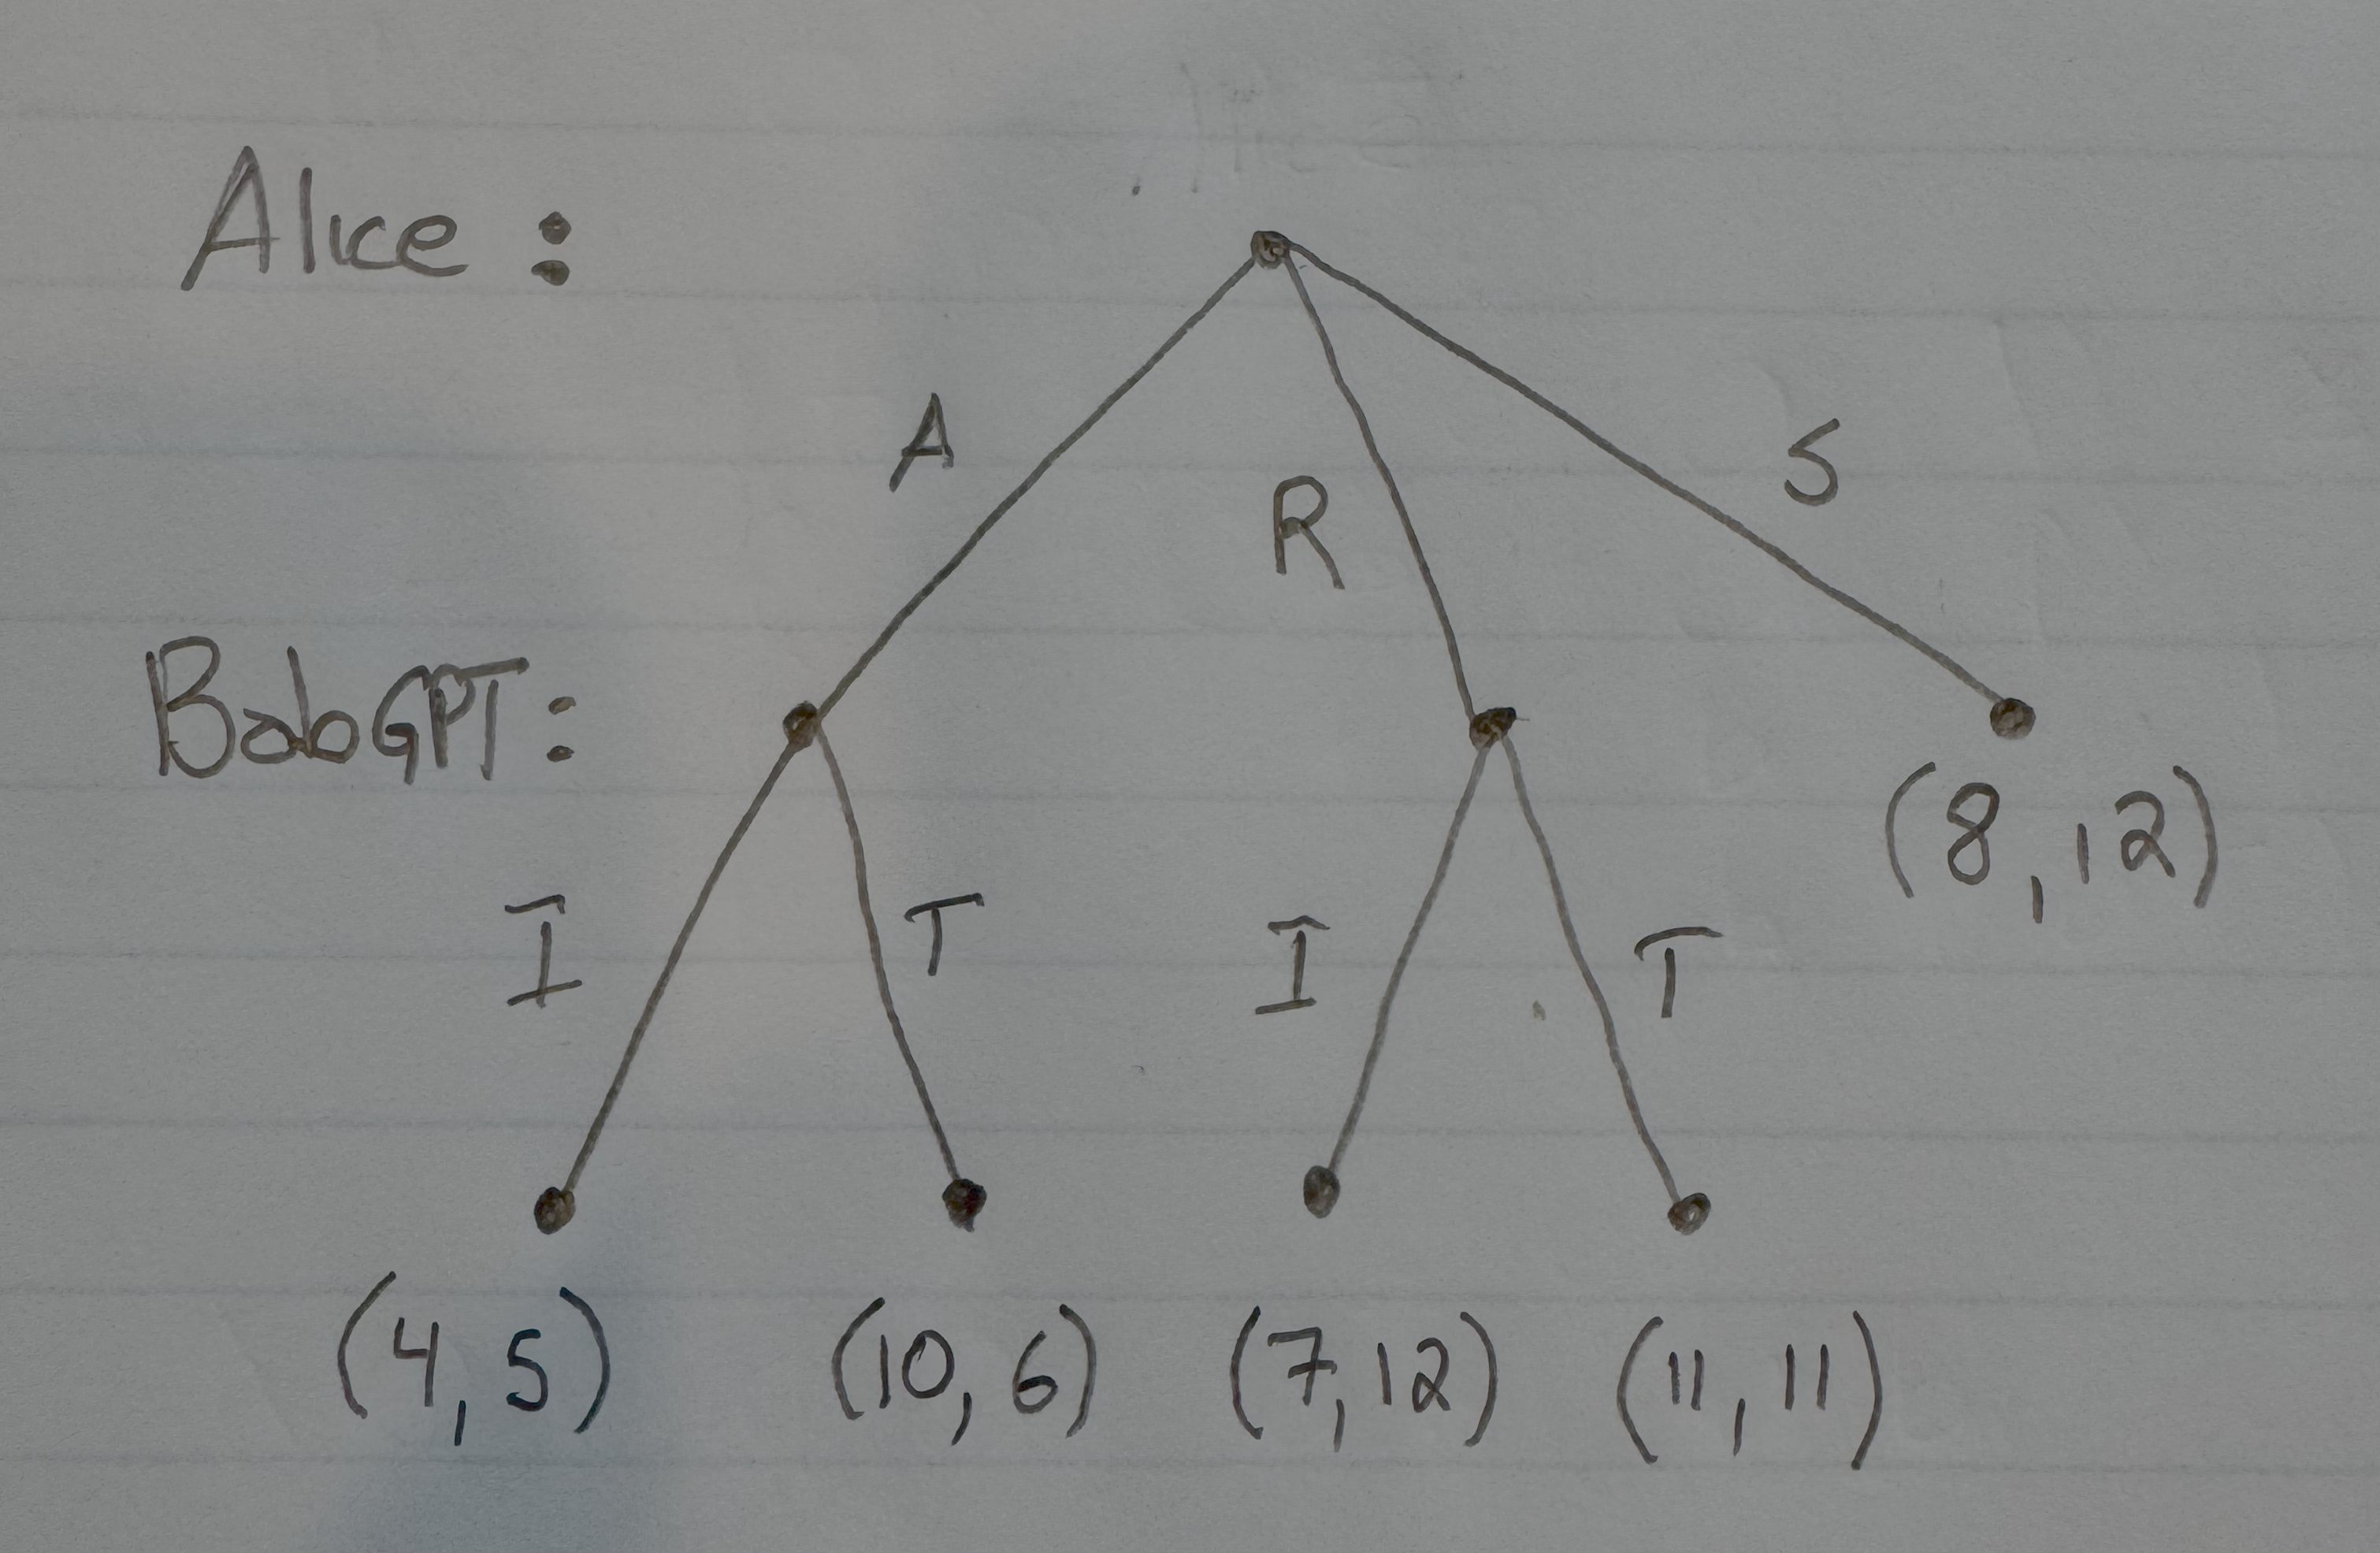
\includegraphics[width=0.6\textwidth]{hw1_problem3_parta.png}
            \caption{Problem 3 Part (a) Extensive form game tree}
            \label{fig:3-a}
        \end{figure}

        \part \textit{Pure strategies and subgame perfect equilibria.} Using first letter of each action for notation, and ordering BobGPTs actions following $A-R$; under Self, the AI does not act:
        \begin{align*}
            s_\text{Alice} &\in \{A, R, S\}\\
            s_\text{BobGPT} &\in \{II, IT, TI, TT\}\\
        \end{align*}
        SPE calculated through backward induction for $\{\Gamma(A), \Gamma(R), \Gamma\}$:
        \begin{align*}
            \Gamma(A):& \left.T\right|_A \text{ with payoffs } (10,6)\\
            \Gamma(R):& \left.I\right|_R \text{ with payoffs } (7,12)\\
            \Gamma:& \left.A\right. \text{ with payoffs } (10, 6)
        \end{align*}
        So $(A, TI)$ is the SPE with payoffs $(10,6)$. The SPE is unique because no payoff was a tie.


        \part \textit{Strategic form payoff matrix.}
        \begin{align*}
            \begin{array}{c|cccc}
                    & II & IT & TI & TT \\ \hline
                A    & (4,5)   & (4,5)   & (10,6)   &  (10,6)  \\
                R    & (7,12)   & (11,11)   &  (7,12)  & (11,11)   \\
                S    & (8,12)   &  (8,12)  &  (8,12)  & (8,12)   \\
            \end{array}
        \end{align*}
        Pure strategy Nash equilibria $\{(S, II), (A, TI)\}$:
        \begin{itemize}
            \item $(S, II)$: BobGPT chooses $II$ $\implies$ Alice chooses $S$ $\implies$ BobGPT doesn't deviate. All other BobGPT choices incentivize Alice to deviate from $S$.
            \item $(A, TI)$: BobGPT chooses $TI$ $\implies$ Alice chooses $A\implies$ BobGPT doesn't deviate. All other BobGPT choices incentivize Alice to deviate from $A$.
            \item No equilibria with Alice choosing $R$: Alice chooses $R\implies$ BobGPT chooses $\{II,TI\}\implies$ Alice chooses $\{S, A\}$ respectively $\implies$ the equilibria above.
            \item No equilibria with BobGPT choosing $TT$: BobGPT chooses $TT\implies$ Alice chooses $R\implies$ see previous bullet.
        \end{itemize}
        
        
        \part \textit{Subgame perfect Nash equilibria.} No, not every Part(c) Nash equilibrium is subgame perfect:
        \begin{itemize}
            \item $s=(A, TI)$ is by Part(b).
            \item $s = (S, II)$ is not since $\left. s\right|_A = I$ where $T$ would lead to a higher payoff ($6>5$). Therefore $s$ is not a Nash equilibrium of subgame $\Gamma(A)$ so it is not subgame perfect by definition.
        \end{itemize} 


        \part \textit{Thinking after review and subgame perfect equilibria.} Thinking after Review fixes Review's payoff to $(11,11)$; BobGPT does not have a decision.
        Strategy profiles are
        \begin{align*}
            s_\text{Alice} &\in \{A, R, S\}\\
            s_\text{BobGPT} &\in \{I, T\}\\
        \end{align*}
        Subgames are $\{\Gamma(A), \Gamma\}$, and through backward induction
        \begin{align*}
            \Gamma(A):& \left.T\right|_A \text{ with payoffs } (10,6)\\
            \Gamma:& \left.R\right. \text{ with payoffs } (11, 11)
        \end{align*}
        So $(R, T)$ is the SPE with payoffs $(11, 11)$. The SPE is unique because no payoff was a tie. Both players benefit relative to ($A, TI$) in Part(b) (Alice: $10\to11$; BobGPT: $6\to11$).

        A non-binding promise of BobGPT to use Thinking after Review would not sustain this outcome: Under Alice's choice of Review, BobGPT's choice of Instant is a best response ($12>11$). And anticipating BobGPT's choice of Instant after Review, Alice's choice of Ask is a best response ($10>7$). 

    \end{parts}

    \question \textbf{Autonomous pricing.}
    \begin{parts}
        \part \textit{Strategic form game.} 
        In any period $t\in[1,T]$ the strategic form game with per-period profit is

        \begin{tabular}{r|cc}
            \textbf{(A,B)} & \textbf{\$10} & \textbf{\$8} \\
            \hline
            \textbf{\$10} & (3,3) & (0,4) \\
            \textbf{\$8} & (4,0) & (2,2) \\
        \end{tabular}
        \begin{itemize}
            \item \textbf{Pure strategy Nash equilibria:} $s^* = (\$8, \$8)$. For seller A the \$8 offer strictly dominates the \$10 offer ($4>3$ when seller B offers \$10; $2>0$ when seller B offers \$8). The symmetric argument holds for seller B. 
            \item \textbf{Mixed strategy Nash equilibria:} None exist.
            \begin{itemize}
                \item As noted above, both players have a strictly dominated strategy, so against any pure strategy, the other player has a unique best response. So any mixed strategy requires both players to randomize. 
                \item Next suppose there exists a mixed strategy Nash equilibrium $(\sigma^*_A, \sigma^*_B)$. Then
                \begin{align*}
                    \operatorname{supp}(\sigma^*_A) = \{\$10, \$8\} \subseteq BR_A(\sigma^*_B) 
                    &\implies u_A(\$10, \sigma^*_B) = u_A(\$8, \sigma^*_B)\\
                    &\implies \mathbb E_{s_B \sim \sigma_B^*}[u_A(\$10, s_B)] = \mathbb E_{s_B \sim \sigma_B^*}[u_A(\$8, s_B)]\\
                    &\implies 3\cdot(1 - \sigma_B^*(\$8)) + 0\cdot\sigma_B^*(\$8) = 4\cdot(1 - \sigma_B^*(\$8)) + 2\cdot\sigma_B^*(\$8)\\
                    &\implies \sigma^*_B(\$8) = -1
                \end{align*}
                A contradiction since we require $\sigma^*_B(\$8)\in(0,1)$. So there is no mixed strategy Nash equilibrium.
                \item This can also be seen by noting that strict dominance against every pure strategy implies strict dominance against any mixture, i.e., $u_A(\$8, \sigma^*_B) > u_A(\$10,\sigma^*_B)\;\forall\;\sigma^*_B$.
            \end{itemize}
        \end{itemize}



        \part \textit{Finite game subgame perfect equilibria.} 
        Let $s^* = (\$8, \$8)_{t\in[1,T]}$ be the strategy profile where both sellers offer \$8 after every history.
        \begin{itemize}
            \item By Part (a), $s^* = (\$8, \$8)$ is a unique pure equilibrium to the stage game, and no mixed equilibrium exists.
            \item By class theorem, if a stage game has a unique Nash equilibrium $a^*$, then its finitely repeated version has a unique SPE, in which players choose $a^*$ in every period regardless of the history. Hence $s^*$ is the unique SPE.
            \item This theorem holds for any finite $T$ and any $\delta\in(0,1)$, so equilibrium behavior does not depend on these values.
            \item In this equilibrium each seller earns 2 per period, so each seller's total discounted payoff is $g_i(s^*) = \sum_{t=1}^{T} \delta^{t-1}\cdot 2$.
        \end{itemize}


        \part \textit{Infinite game strategy profile.}
        A strategy profile $s^*$ is an SPE if and only if no player can gain by deviating from $s^*$ in a single stage and conforming to $s^*$ thereafter. 

        Consider seller A choosing deviation at time $\bar t$; assume $s^*_B$. Everything before $\bar t$ is equivalent between comply and deviation so we ignore it. For each state, seller A's payoffs by choice (comply, deviate) and the no-deviation condition are below
        \begin{table}[h!]
        \centering
        \begin{tabular}{l|lll}
            \textbf{Current state} & \textbf{Comply} & \textbf{Deviate} & \textbf{Condition} \\
            \hline
            \textbf{No punishment} 
                & $\sum_{t=\bar t}^\infty 3\delta^{t-1}$ 
                & $4\delta^{\bar t-1} + \sum_{t=\bar t+1}^{\bar t+2} 2\delta^{t-1} + \sum_{t=\bar t+3}^\infty 3\delta^{t-1}$
                & $\delta^2 + \delta - 1 \geq 0$ \\
            \textbf{Two punishment} 
                & $\sum_{t=\bar t}^{\bar t+1} 2\delta^{t-1} + \sum_{t=\bar t+2}^\infty 3\delta^{t-1}$  
                & $0\delta^{\bar t-1} + \sum_{t=\bar t+1}^{\bar t+2} 2\delta^{t-1} + \sum_{t=\bar t+3}^\infty 3\delta^{t-1}$ 
                & $\delta^2 +2 \geq 0$\\
            \textbf{One punishment} 
                & $2\delta^{\bar t-1} + \sum_{t=\bar t+1}^\infty 3\delta^{t-1}$  
                & $0\delta^{\bar t-1} + \sum_{t=\bar t+1}^{\bar t+2} 2\delta^{t-1} + \sum_{t=\bar t+3}^\infty 3\delta^{t-1}$
                & $\delta^2 + \delta + 2 \geq 0$
        \end{tabular}
        \end{table}
        This analysis covers all histories because each history leads to these three states for different $\bar t$. Looking more closely at these no-deviation conditions:
        \begin{itemize}
            \item No punishment ($\delta^2 + \delta - 1 \geq 0$) is satisfied for $\delta \notin (\tfrac{-1-\sqrt5}{2}, \tfrac{-1+\sqrt5}{2} )$ and $\delta \in (0,1)$. Together this requirement is $\delta \in [\tfrac{-1+\sqrt5}{2}, 1)$
            \item Two punishment ($\delta^2 +2 \geq 0$) is satisfied for all $\delta \in \mathbb R$ and therefore all $\delta \in(0,1)$.
            \item One punishment ($\delta^2 + \delta + 2 \geq 0$) is satisfied for all $\delta\in\mathbb R$ and therefore all $\delta \in(0,1)$.
        \end{itemize}
        Seller A has no incentive to deviate from the strategy profile under the conditions above. By symmetry, the same holds for seller B. So this strategy profile is an SPE when $\delta \in [\tfrac{-1+\sqrt5}{2}, 1)$.

        At the threshold value $\delta = \tfrac{-1+\sqrt5}{2}$, seller $i$ is indifferent between complying and deviating from the no-punishment state so this value still permits the SPE. Neither seller ever has an incentive to deviate from the two-punishment and one-punishment states. 



        \part \textit{Permanent punishment.} Following the template of above
        \begin{table}[h!]
        \centering
        \begin{tabular}{l|lll}
            \textbf{Current state} & \textbf{Comply} & \textbf{Deviate} & \textbf{Condition} \\
            \hline
            \textbf{No punishment} 
                & $\sum_{t=\bar t}^\infty 3\delta^{t-1}$ 
                & $4\delta^{\bar t-1} + \sum_{t=\bar t+1}^{\infty} 2\delta^{t-1}$
                & $\delta \geq \frac{1}{2}$ \\
            \textbf{Permanent punishment} 
                & $\sum_{t=\bar t}^{\infty} 2\delta^{t-1}$  
                & $0\delta^{\bar t-1} + \sum_{t=\bar t+1}^{\infty} 2\delta^{t-1}$ 
                & $2 \geq 0$\\
        \end{tabular}
        \end{table}
        \begin{itemize}
            \item No punishment is satisfied for $\delta \geq \frac{1}{2}$ and $\delta \in (0,1)$. Together this requirement is $\delta \in [\frac{1}{2}, 1)$.
            \item Permanent punishment is satisfied trivially ($2\geq 0$) and therefore for all $\delta \in(0,1)$.
        \end{itemize}
        This strategy profile permits an SPE for $\delta \in [\frac{1}{2}, 1)$. Comparing to Part(c), $\tfrac{-1+\sqrt5}{2} > \frac{1}{2}$, so the range of discount factors for permanent punishment strategy profile is larger than for the short-term punishment strategy profile. 
        
        Why? In both cases, deviating once gives you a one-period payment of 4 and then payments of 2 for the next two periods. The difference between the strategy profiles is what happens from the third period onward: the short punishment returns to an infinite stream of 3, while the permanent punishment stays at 2. The deviator's payoffs are lower under permanent punishment (deviating is more costly) so the seller needs a higher discount (lower delta) on the future to be willing to deviate.
        
        Neither rule can sustain (\$10,\$10) in a finite game, by the proof in Part(b). This can also be seen clearly by applying the one-shot deviation test to the final period $T$. There's no threat of punishment in this interval so deviating to \$8 pays \$1 at no cost and is the best response; this is a deviation from both proposed strategies. 
    \end{parts}
    
\end{questions}
\end{document}